\chapter{X-Ray Tracking}
\label{c:xray.track}

\bmad can track both charged particles and X-rays. This chapter deals
with X-rays. Charged particles are handled in chapter~\sref{c:charged.track}.

%-------------------------------------------------------------------------
%-------------------------------------------------------------------------
\section{Tracking with Non-Zero Offsets, Pitches, or Tilt}
\label{s:photon.ele.coords}

\index{element coordinates}
\index{crystal}\index{mirror}\index{multilayer_mirror}
As explained in section~\sref{s:ele.coords}, \vn{element} coordinates
are used for tracking calculations.

For \vn{crystal} (\sref{s:crystal}), \vn{mirror} (\sref{s:mirror}),
and \vn{multilayer_mirror} (\sref{s:multilayer}) elements, the
``kinked'' reference trajectory through the element complicates the
calculation. For these elements, there are three coordinate systems
attahed to the element as shown in \fig{f:photon.ele.coords}. Besides
the \vn{element entrance} and \vn{element exit} coordinates, there are
\vn{element surface} coordinates with $z$ perpendicular to the surface
pointing inward.

Tracking a particle through an element is therefore a three
step transformation:
\begin{enumerate}
\item
At the entrance end of the element, transform from the laboratory
reference coordinates to the element's \vn{entrance} or \vn{surface}
coordinates.
\item
Track through the element ignoring any misalignments.
\item
At the exit end of the element, transform from the element coordinates
to the \vn{laboratory} \vn{exit} coordinates.
\end{enumerate}


%-------------------------------------------------------------------------

\begin{figure}[tb]
  \centering
  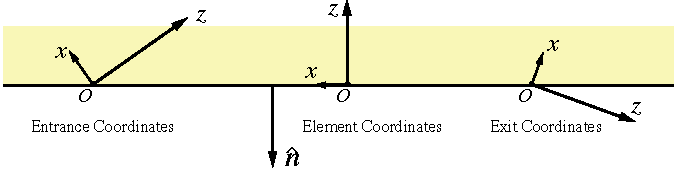
\includegraphics[width=5in]{photon-ele-coords.pdf}
  \caption[Crystal, Mirror, and Multilayer_Mirror Element Coordinates.]
{The three element coordinate systems for \vn{crystal} (Bragg
configuration), \vn{mirror}, and \vn{multilayer_mirror} elements.  The
origin $\Bf O$ of all three are the same but are shown spread out for
clarity.  $\bfhat n$ is the normal to the element surface.}
  \label{f:photon.ele.coords}.
\end{figure}

%-------------------------------------------------------------------------
\subsection{Transform from Laboratory Entrace to Element Coordinates}

For elements that have a reference orbit kink
(\sref{s:photon.ele.coords}), the element coordinates here are the
\vn{surface} coordinates. Otherwise the element coordinates are
the entrance coordinates.

\begin{enumerate}
\item
Apply offsets
\begin{align}
  x_1    &= x_0 - x_{\mbox{off}}
  y_1    &= y_0 - y_{\mbox{off}}
  z_1    &= z_0 - z_{\mbox{off}}
\end{align}
\item
Apply pitches
\begin{align}
  x_2    &=  x_1    \, \cos\theta_t + y_1    \, \sin\theta_t \CRNO
  p_{x2} &=  p_{x1} \, \cos\theta_t + p_{y1} \, \sin\theta_t \CRNO
  y_2    &= -x_1    \, \sin\theta_t + y_1    \, \cos\theta_t \\
  p_{y2} &= -p_{x1} \, \sin\theta_t + p_{y1} \, \cos\theta_t \nonumber
\end{align}
\end{enumerate}

%-------------------------------------------------------------------------
\subsection{Transform from Element Exit to Laboratory Coordinate}

The back transformation from element to laboratory coordinates is
accomplished by the transformation
\begin{enumerate}
\item
Apply any tilt $\theta_t$
\begin{align}c
  x_1    &=  x_0    \, \cos\theta_t - y_0    \, \sin\theta_t \CRNO
  p_{x1} &=  p_{x0} \, \cos\theta_t - p_{y0} \, \sin\theta_t \CRNO
  y_1    &=  x_0    \, \sin\theta_t + y_0    \, \cos\theta_t \\
  p_{y1} &=  p_{x0} \, \sin\theta_t + p_{y0} \, \cos\theta_t \nonumber
\end{align}
\item
Apply offsets and pitches
\begin{align}
  x_2    &= x_1 + x_{\mbox{off}} + \frac{L}{2} x'_{pitch}     \CRNO
  p_{x2} &= p_{x1} + (1 + p_{z1}) \, x'_{pitch}        \CRNO
  y_2    &= y_1 + y_{\mbox{off}} + \frac{L}{2} y'_{pitch}     \\
  p_{y2} &= p_{x1} + (1 + p_{z1}) \, y'_{pitch}        \CRNO
  z_2    &= z_1 + x'_{pitch} \, x_1 + y'_{pitch} \, y_1 - 
    \frac{L}{4} (x^{\prime2}_{pitch} + y^{\prime2}_{pitch})      \nonumber
\end{align}
\item
Track as in a drift a distance \vn{-z_offset_tot}.
\end{enumerate}

%-------------------------------------------------------------------------
%-------------------------------------------------------------------------
\section[Mirror and Crystal Element Transformation]
{Transformation for Mirror and Crystal Elements Between 
Laboratory and Element Coordinates}
\label{s:photon.lab.ele}

\index{mirror}\index{crystal}

%-------------------------------------------------------------------------
\subsection{Transformation from Laboratory to Element Coordinates}
\label{ss:crystal.trans.le}

\index{z_offset_tot}
With photons, the intensities must also be transformed.
The transformation from the the entrance laboratory coordinates to
the entrance element coordinates is:
\begin{enumerate}
\item
Track as in a drift a distance \vn{z_offset_tot}.
\item
\index{x_offset}\index{x_pitch}\index{y_offset}\index{y_pitch}
Apply offsets and pitches: The effective ``length'' of the element is
zero (\sref{s:mirror.coords}) so the origin of the element coordinates
is the same point around which the element is pitched so
\begin{align}
  x_1    &= x_0 - x_{\mbox{off}} \CRNO
  p_{x1} &= p_{x0} - (1 + p_{z0}) \, x'_{pitch} \CRNO
  y_1    &= y_0 - y_{\mbox{off}} \\
  p_{y1} &= p_{x0} - (1 + p_{z0}) \, y'_{pitch} \CRNO
  z_1    &= z_0 + x'_{pitch} \, x_1 + y'_{pitch} \, y_1 \nonumber
\end{align}
where $x_{\mbox{off}} \equiv \vn{x_offset}$, $x'_{pitch} \equiv \vn{x_pitch}$, etc.
\item
Apply \vn{ref_tilt} and \vn{tilt}:
\begin{align}
  \begin{pmatrix} x_2 \\ y_2 \end{pmatrix} &=
    \bfR (\theta_{tot}) \,   
  \begin{pmatrix} x_1 \\ y_1 \end{pmatrix} \CRNO
  \begin{pmatrix} p_{x2} \\ p_{y2} \end{pmatrix} &=
    \bfR (\theta_{tot}) \, 
  \begin{pmatrix} p_{x1} \\ p_{y1} \end{pmatrix} \label{xyrtxy} \\ 
  \begin{pmatrix} \bfE_{x2} \\ \bfE_{y2} \end{pmatrix} &=
    \bfR (\theta_{tot}) \,   \begin{pmatrix} \bfE_{x1} \\ \bfE_{y1} \end{pmatrix} \nonumber
\end{align}
where $\bfE$ is shorthand notation for
\Begineq
  \bfE \equiv E \, e^{i \, \phi}
\Endeq
with $E$ being the field intensity and $\phi$ being the field phase angle.
In the above equations $\bfR$ is the rotation matrix
\Begineq
  \bfR(\theta) = \begin{pmatrix} \cos\theta & \sin\theta \\ -\sin\theta & \cos\theta \end{pmatrix}
\Endeq
\index{tilt}\index{ref_tilt}\index{tilt_corr}
with $\theta_{tot}$ being 
\Begineq
  \theta_{tot}  = 
  \begin{cases}
    \vn{ref_tilt} + \vn{tilt} + \vn{tilt_corr} & \vn{for crystal elements} \\
    \vn{ref_tilt} + \vn{tilt} & \vn{for mirror elements}
  \end{cases}
  \label{tttt}
\Endeq
The \vn{tilt_corr} correction is explained in \sref{ss:crystal.trans}.
\end{enumerate}

%-------------------------------------------------------------------------
\subsection{Transformation from Element to Laboratory Coordinates}
\label{ss:crystal.trans.el}

The back transformation from exit element coordinates to exit
laboratory coordinates is accomplished by the transformation
  \begin{enumerate}
  \item
Apply \vn{ref_tilt} and \vn{tilt}: \vn{ref_tilt} rotates the exit
laboratory coordinates with respect to the exit element coordinates in
the same way \vn{ref_tilt} rotates the entrance laboratory coordinates
with respect to the entrance element coordinates. The forward and back
transformations are thus just inverses of each other.  With
\vn{tilt}, this is not true. \vn{tilt}, unlike \vn{ref_tilt}, does
not rotate the output laboratory coordinates.  There is the further
complication in that \vn{tilt} is a rotation about the {\em
entrance} laboratory coordinates. The first step is to express
\vn{tilt} with respect to the exit coordinates. This is done with
the help of the $\bfS$ matrix of \Eq{ltl} with $\alpha$ given by
\Eq{agg}. The effect of the \vn{tilt} can be modeled as a rotation
vector $\Bf e_{in}$ in the entrance laboratory coordinates pointing
along the $z$-axis
\Begineq
 \Bf e_{in} = (0, 0, \mbox{tilt})
\Endeq
In the exit laboratory coordinates, the vector $\Bf e_{out}$ is
\Begineq
  \Bf e_{out} = \bfS \, \Bf e_{in}
\Endeq
The $z$ component of $\Bf e_{out}$ combines with \vn{ref_tilt} to give
the transformation
\begin{align}
  \begin{pmatrix} x_2 \\ y_2 \end{pmatrix} &=
    \bfR (-\theta_{t}) \,   \begin{pmatrix} x_1 \\ y_1 \end{pmatrix} \CRNO
  \begin{pmatrix} p_{x2} \\ p_{y2} \end{pmatrix} &=
    \bfR (-\theta_{t}) \,   \begin{pmatrix} p_{x1} \\ p_{y1} \end{pmatrix} \\
  \begin{pmatrix} \bfE_{x2} \\ \bfE_{y2} \end{pmatrix} &=
    \bfR (-\theta_{t}) \,   \begin{pmatrix} \bfE_{x1} \\ \bfE_{y1} \end{pmatrix} \nonumber
\end{align}
where $\theta_t$ is $\mbox{ref_tilt} + \Bf e_{out,z}$. The $x$ and $y$ components
of $\Bf e_{out}$ give rotations around the $x$ and $y$ axes
\begin{align}
  p_{x3} &= p_{x2} - \Bf e_{out,y} \CRNO
  p_{y3} &= p_{y2} + \Bf e_{out,x} \\
  z_3    &= z_2 + x_2 \, \Bf e_{out,y} - y_2 \, \Bf e_{out,x}
\end{align}
  \item
Apply pitches: Since pitches are defined with
respect to the entrance laboratory coordinates, they have to be
translated to the exit laboratory coordinates
\Begineq
  \bfP_{out} = \bfS \, \bfP_{in}
\Endeq
where $\bfP_{in} = (x'_{pitch}, y'_{pitch}, 0)$ is the pitch vector in
the entrance laboratory frame and $\bfP_{out}$ is the vector in the exit
laboratory frame. The transformation is then
\begin{align}
  p_{x4} &= p_{x3} - \bfP_{out,y} \CRNO
  p_{y4} &= p_{y3} + \bfP_{out,x} \\
  z_4    &= z_3 + x_3 \, \bfP_{out,y} - y_3 \, \bfP_{out,x}
\end{align}
  \item
Apply offsets: Again, offsets are defined with respect to the
entrance laboratory coordinates. Like pitches, the translation is
\Begineq
  \bfO_{out} = \bfS \, \bfO_{in}
\Endeq
where $\bfO_{in} = (x_{\mbox{off}}, y_{\mbox{off}}, s_{\mbox{off}})$ is the offset in the
entrance laboratory frame. The transformation is
\begin{align}
  x_5 &= x_4 + \bfO_{out,x} - p_{x4} \, \bfO_{out,z} \CRNO
  y_5 &= y_4 + \bfO_{out,y} - p_{y4} \, \bfO_{out,z} \\
  z_5 &= z_4 + \bfO_{out,z} 
\end{align}
  \end{enumerate}

%-------------------------------------------------------------------------

\begin{figure}[tb]
  \centering
  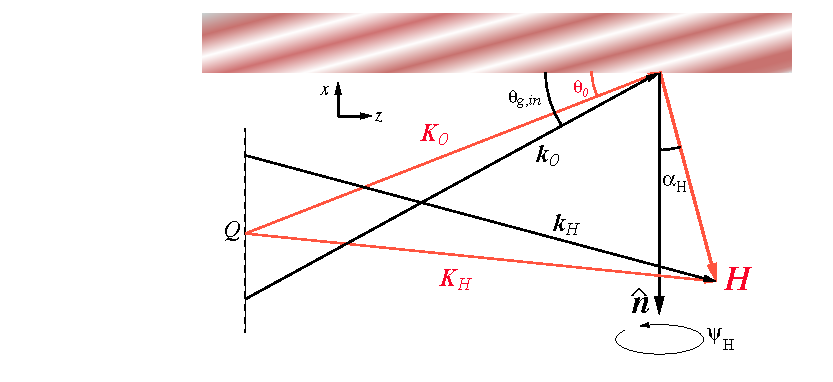
\includegraphics[width=5in]{crystal-diffraction.pdf}
  \caption[Reference trajectory reciprocal space diagram for crystal diffraction.]
{Reference trajectory reciprocal space diagram for for A) Bragg
diffraction and B) Laue diffraction. The bar over the vectors
indicates that they refer to the reference trajectory. The $x$-$z$
coordinates shown are the element surface coordinates. All points in the
diagram are in the plane of the paper except for the tip of $\bfH$.
$\bfKbar_{0}$, and $\bfKbar_{H}$ are the wave vectors inside the
crystal and $\bfkbar_{0}$ and $\bfkbar_{H}$ are the wave vectors
outside the crystal. The reference photon traveling along the
reference trajectory has $\bfKbar_0$ and $\bfKbar_H$ originating at
the $Q$ point. For Laue diffraction, the crystal faces are assumed
parallel.  For Bragg diffraction the crystal normal is in the $-\bfhat
x$ direction while for Laue diffraction the crystal normal is in the
$-\bfhat z$ direction
  }
  \label{f:crystal.diffraction}
\end{figure}

%-------------------------------------------------------------------------
\section{Coherent and Incoherent Tracking}
\label{s:coherent.track}

\index{coherent tracking}\index{incoherent tracking}
\bmad can track photons either \vn{coherenly} or \vn{incoherently}.


%-------------------------------------------------------------------------
%-------------------------------------------------------------------------
\section{Crystal Element Tracking}
\label{s:crystal.tracking}

\textit{\large [Crystal tracking developed by Jing Yee Chee, Ken Finkelstein, and David Sagan]}

Crystal diffraction is modeled using dynamical diffraction theory. The
notation here follows Batterman and Cole\cite{b:batterman}.  The
problem can be divided up into two parts. First the reference
trajectory must be calculated. This means calculating the incoming
grazing angle $\theta_{B,in}$ and outgoing grazing angle
$\theta_{B,out}$ as well as calculating the transformations between
the various coordinate systems. This is done in \sref{ss:crystal.ref},
\sref{ss:crystal.trans}, and \sref{ss:laue.ref}.  The second part
is the actual tracking of the photon and this is covered in
\sref{ss:bragg.track} and \sref{ss:laue.track}.

%-------------------------------------------------------------------------
\subsection{Calculation of Entrance and Exit Bragg Angles}
\label{ss:crystal.ref}

\fig{f:crystal.diffraction} shows the geometry of the
problem. The bar over the vectors indicates that they refer to the
reference trajectory. The reference trajectory is calculated such that
the reference photon will be in the center of the Darwin curve. That
is, the internal wave vectors $\bfKbar_0$ and $\bfKbar_H$ originate
from the $Q$ point (See \cite{b:batterman} Figs.~8 and 29).

The external wave vectors $\bf k_0$, and $\bf k_H$ and the internal wave vectors
have magnitude
\begin{align}
  |\bf k_0| &= |\bf k_H| = \frac{1}{\lambda} 
  \label{kk1l1} \\
  |\bfKbar_0| &= |\bfKbar_H| = \frac{1}{\lambda \, (1 + \delta)}
  \label{kk1l2}
\end{align}
where $\lambda$ is the wavelength, and $\delta$ is
\Begineq
  \delta = \frac{\lambda^2 r_e}{2 \, \pi \, V} \, |F_0|
\Endeq
with $r_e$ being the classical electron radius, $V$ the unit cell
volume, and $F_0$ the $F_{(0,0,0)}$ structure factor. 

In element surface coordinates (which will be the coordinate system used
henceforth), $\bfkbar_0$ lies in the $x$-$z$ plane. $\bfKbar_0$ is
related to $\bfkbar_0$ via Batterman Eq.~(25)
\Begineq
  \bfK_0 = \bfk_0 + q_0 \, \bfhat n
  \label{kkqn1}
\Endeq
where the value of $q_0$ is to be determined. Here, and in equations
below, if the equation is true in general, and not just for the
reference trajectory, the bar superscript is dropped.

Since $\bfhat n$ is in the $-\bfhat x$ direction, $\bfKbar_0$ is also
in the $x$-$z$ plane. Thus $\bfkbar_0$ and $\bfKbar_0$ can be written
in the form
\begin{alignat}{3}
  \bfkbar_0 &= \frac{1}{\lambda} \, 
    \begin{pmatrix}
    -\cos\theta_{B,in} \\
    0 \\
    \sin\theta_{B,in}
    \end{pmatrix}
  \; , & \qquad
  \bfKbar_0 &= \frac{1}{\lambda \, (1 + \delta)} \, 
    \begin{pmatrix}
    -\cos\theta_0 \\
    0 \\
    \sin\theta_0
    \end{pmatrix}
  & \qquad &\mbox{[Bragg]} \CRNO
  \bfkbar_0 &= \frac{1}{\lambda} \, 
    \begin{pmatrix}
    \sin\theta_{B,in} \\
    0 \\
    \cos\theta_{B,in}
    \end{pmatrix}
  \; , & \qquad
  \bfKbar_0 &= \frac{1}{\lambda \, (1 + \delta)} \, 
    \begin{pmatrix}
    \sin\theta_0 \\
    0 \\
    \cos\theta_0
    \end{pmatrix}
  &\qquad & \mbox{[Laue]} 
  \label{k1lst}
\end{alignat}
Where, as shown in \fig{f:crystal.diffraction}, $\theta_{B,in}$, and
$\theta_0$ are the angles of $\bfkbar_0$ and $\bfKbar_0$ with respect
to the $x$-axis for Bragg reflections and with respect to the $z$-axis
for Laue reflection.

$\alpha_H$ (\vn{alpha_angle}) is the angle that $\bfH$ makes with
respect to the $-\bfhat z$ axis and $\psi_H$ (\vn{psi_angle}) is the
rotation of $\bfH$ around the $-\bfhat z$ axis such that for $\psi_H =
0$, $\bfH$ is in the $x$-$z$ plane and oriented as shown in
\fig{f:crystal.diffraction}. Thus
\Begineq
  \bfH 
  \equiv \frac{1}{d} \, \bfhat{H} 
  = \frac{1}{d}
    \begin{pmatrix} 
       -\sin \alpha_H \, \cos \psi_H \\ \sin \alpha_H \, \sin \psi_H \\ -\cos \alpha_H
    \end{pmatrix}
  \label{h1daa}
\Endeq
where $\bfhat{H}$ is $\bfH$ normalized to 1.

The vectors $\bfK_0$ and $\bfH$ must add up to the reciprocal lattice vector $\bfK_H$
\Begineq
  \bfK_H = \bfK_0 + \bfH
  \label{kkh}
\Endeq
Taking the length of both sides of this equation and using
\Eqs{kk1l2}, \eq{k1lst}, and \eq{h1daa} gives for
$\theta_0$
\Begineq
  \sin \theta_0 = 
  \begin{dcases}
    \dsfrac{-\beta \, \what{H}_z - \what{H}_x \, \sqrt{\what{H}_x^2 + \what{H}_z^2 - \beta^2}}
    {\what{H}_x^2 + \what{H}_z^2} & \vn{Bragg} \\
    \dsfrac{-\beta \, \what{H}_x + \what{H}_z \, \sqrt{\what{H}_x^2 + \what{H}_z^2 - \beta^2}}
    {\what{H}_x^2 + \what{H}_z^2} & \vn{Laue}
  \end{dcases}
\Endeq
where
\Begineq
  \beta \equiv \frac{\lambda \, (1 + \delta)}{2 \, d}
\Endeq
Once $\theta_0$ has been calculated, $\theta_{B,in}$ can be calculated from \Eq{kkqn1}
\begin{align}
  \cos\theta_{B,in} &= \frac{\cos\theta_0}{1 + \delta} \quad [\mbox{Bragg}] \\
  \sin\theta_{B,in} &= \frac{\sin\theta_0}{1 + \delta} \quad [\mbox{Laue}] 
\end{align}

The outgoing reference wave vector $k_H$ is computed using the equation
\Begineq
  \bfK_H = \bfk_H + q_H \, \bfhat n
  \label{kkqn2}
\Endeq
Using this with \Eqs{h1daa} and \eq{kkh} gives
\begin{align}
  \kbar_{H,x} &= \Kbar_{H,z} = \frac{1}{d} \, \what{H}_x + \kbar_{0,x} \\
  \kbar_{H,y} &= \Kbar_{H,y} = \frac{1}{d} \, \what{H}_y 
  \label{k1dapl} \\
  \kbar_{H,z} &= \sqrt{\frac{1}{\lambda^2} - \kbar_{H,x}^2 - \kbar_{H,y}^2} \nonumber
\end{align}

The total bending angle of the reference trajectory is then
\Begineq
  \theta_{bend} = \tan^{-1} 
  \left( \frac{ | \bfkbar_0 \times \bfkbar_H | }{\bfkbar_0 \cdot \bfkbar_H} \right)
\Endeq
The outgoing Bragg angle $\theta_{B,out}$ is then {\em defined} to be
the difference between the total bend angle and the entrance Bragg angle.
\Begineq
  \theta_{B,out} \equiv \theta_{bend} - \theta_{B,in}
\Endeq

%-------------------------------------------------------------------------
\subsection{Crystal Coordinate Transformations}
\label{ss:crystal.trans}

There are four transformations needed between coordinates
denoted by $\Bf\Sigma_1$, $\Bf\Sigma_2$, $\Bf\Sigma_3$, and $\Bf\Sigma_4$
\begin{example}
  \(\Bf\Sigma_1\)  Transform from laboratory entrance to element entrance coordinates.  
  \(\Bf\Sigma_2\)  Transform from element entrance to surface coordinates.  
  \(\Bf\Sigma_3\)  Transform from surface to element exit coordinates.  
  \(\Bf\Sigma_4\)  Transform from element exit to laboratory exit coordinates.  
\end{example}
The total transformation is just the map represented by $\bfS$ and
$\bfV$ of \Eqs{vwlv} and \eq{wws}
\Begineq
  [\bfS, \bfV] = \Bf\Sigma_4 \, \Bf\Sigma_3 \, \Bf\Sigma_2 \, \Bf\Sigma_1
\Endeq

\index{tilt_corr}\index{crystal!tilt correction}
The transformation $\Bf\Sigma_1$ is given in
\sref{ss:crystal.trans.le} and the transformation $\Bf\Sigma_4$ is
given in \sref{ss:crystal.trans.el}. In general, the transformation
$\Bf\Sigma_1$ needs a ``tilt correction'' (\Eq{tttt}), as explained
below, when $\psi_H$ is nonzero.  [The exception is when the
\vn{undiffracted} or \vn{forward diffracted} beam is tracked with Laue
geometry. In these cases, no tilt correction is needed.] Since this
tilt correction is independent of any misalignments, the tilt
correction calculation proceeds assuming here that there are no
misalignments. The finite $\bfV$ due to the finite crystal thickness
in Laue diffraction will also be ignored for the moment.

Without misalignments, and with $\psi_H$ zero, the transformation
$\Bf\Sigma_1$ is, as it is for every other type of element,
just the unit matrix. 
\Begineq
  \Bf\Sigma_1 = \bfI
\Endeq
That is, the two coordinate systems are
identical. Furthermore, the transformation $\Bf\Sigma_2$ from element
entrance coordinates to surface coordinates is a rotation around the $y$
axis
\begin{align}
  \Bf\Sigma_2 &= \bfR_y(\theta_{B,in}) \equiv \begin{pmatrix}
     \cos\theta_{B,in} & 0 & \sin\theta_{B,in} \\
     0                 & 1 & 0                 \\
    -\sin\theta_{B,in} & 0 & \cos\theta_{B,in} \\
  \end{pmatrix}
  \qquad &\mbox{[Laue]}
  \label{mt0t010} \\
  &= \bfR_y(\theta_{B,in} - \frac{\pi}{2})
  \qquad &\mbox{[Bragg]} \nonumber
\end{align}
The transformation from element surface coordinates to element exit
coordinates, $\Bf\Sigma_3$, is another rotation around the $y$ axis 
\begin{align}
  \Bf\Sigma_3 &= \bfR_y(\theta_{B,out})
  \qquad &\mbox{[Laue]} \\
  &= \bfR_y(\theta_{B,out} + \frac{\pi}{2})
  \qquad &\mbox{[Bragg]} \nonumber
\end{align}
and the transformation from element exit coordinates
to laboratory exit coordinates, $\Bf\Sigma_{out}$ is the unity matrix
\Begineq
  \Bf\Sigma_4 = \bfI
\Endeq
Thus, the combined transformation $\bfS$ from laboratory entrance to
laboratory exit coordinates is a rotation around the $y$ axis of
$\theta_{B,in}+\theta_{B,out}$ as explained in section
\sref{s:global}
\Begineq
  \bfS = \Bf\Sigma_4 \, \Bf\Sigma_3 \, \Bf\Sigma_2 \, \Bf\Sigma_1 
  = \bfR_y(\theta_{B,in}+\theta_{B,out})
\Endeq

\index{ref_tilt}\index{psi_angle}
When $\psi_H$ is non-zero, the situation is complicated since, if
$\bfS$ as calculated above is used, the vector $\bfkbar_H$ would be
bent out of the $x$-$z$ plane even though it has been assumed that the
\vn{ref_tilt} $\theta_t$ is zero. But $\bfkbar_H$ points in the same direction
as the $z$ axis of the outgoing reference trajectory. Furthermore, by
{\em definition}, the reference trajectory has the form given by
\Eq{lrca1} with the $\bfT$ matrix depending only upon the \vn{ref_tilt}
parameter (which is here taken to be zero). To satisfy \Eq{lrca1}, the
crystal must be reorientated to keep the $\bfk_H$ vector in the
$x$-$z$ plane of the laboratory entrance coordinates.  The
reorientation is done by rotating the crystal about the laboratory
entrance $\Bf z$ axis by an amount $\theta_{corr}$ (\vn{tilt_corr}).

With this tilt correction the transformation $\Bf\Sigma_1$ is a
rotation about the $z$ axis
\Begineq
  \Bf\Sigma_1 = 
  \begin{pmatrix}
    \cos\theta_{corr} & -\sin\theta_{corr} & 0 \\
    \sin\theta_{corr} &  \cos\theta_{corr} & 0 \\
    0                 &  0                 & 1                
  \end{pmatrix}
\Endeq
To calculate a value for $\theta_{corr}$, note that
the transformation $\Bf\Sigma_2$ from element entrance coordinates to element surface
coordinates is not affected by a finite $\psi_H$ and so \Eq{mt0t010}
is unmodified. The $\bfk_H$ vector, expressed in laboratory entrance
coordinates, is $\Bf\Sigma_1^{-1} \, \Bf\Sigma_2^{-1} \, \bfk_H$ where the
components of $\bfk_H$ are given by \Eq{k1dapl}. To
satisfy \Eq{lrca1}, this vector must have zero $y$ component
\Begineq
  \left( \Bf\Sigma_1^{-1} \, \Bf\Sigma_2^{-1} \, \bfk_H \right) \cdot
  \begin{pmatrix} 0 \\ 1 \\ 0 \end{pmatrix}
  = 0
\Endeq
Solving gives
\Begineq
  \theta_{corr} = \tan^{-1} 
  \frac{k_{H,y}}{k_{H,z} \, \sin\theta_{B,in} - k_{H,x} \, \cos\theta_{B,in}}
\Endeq
The transformation $\Bf\Sigma_3$ from element surface coordinates to
element exit coordinates is now obtained by requiring that the total
transformation from laboratory entrance to laboratory exit coordinates
be the $\bftilde S$ matrix given in \Eq{lrca1}
\Begineq
  \Bf\Sigma_3 \, \Bf\Sigma_2 \, \Bf\Sigma_1 = 
  \begin{pmatrix}
    \cos\theta_{bend} & 0 & -\sin\theta_{bend} \\
    0          & 1 & 0           \\
    \sin\theta_{bend} & 0 & \cos\theta_{bend}
  \end{pmatrix}
\Endeq
In the above equation, the transformation $\Bf\Sigma_4$ has been
dropped since it is the unit matrix independent of $\psi_H$.

For Laue diffraction when the non-diffracted beam is tracked, the exit
coordinate system corresponds to the entrance coordinate system. That
is, $\bfV$ is the unit matrix. In this case, there is no tilt
correction and $\Bf\Sigma_3 = \bfR_y(-\theta_{B,in})$ is just the
inverse of $\Bf\Sigma_2$.

%-------------------------------------------------------------------------

\begin{figure}
\centering
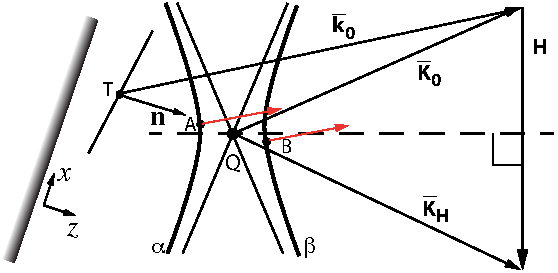
\includegraphics[width=4in]{crystal-energy.pdf}
  \caption[Energy flow for Laue diffraction]{
Energy flow for Laue diffraction for a given tie point is
perpendicular to the dispersion serface (red arrows).
  }
\label{f:crystal.energy}
\end{figure}

%-------------------------------------------------------------------------
\subsection{Laue Reference Orbit}
\label{ss:laue.ref}

For Laue diffraction, with the reference orbit following the
\vn{undiffracted} beam, the reference orbit at the exit surface is
just the extension of the reference orbit at the entrance
surface. Since the reference orbit's direction is $\bfkbar_0$.  the
reference orbit displacement vector $\bfL$ (cf.~\Eq{vwlv}) is given by
\Begineq
  \bfL = \frac{d\bfkbar_0 \, ( d\bfkbar_0 \cdot \Bf t )}{|d\bfkbar_0|^2}
\Endeq
where
\Begineq
  \Bf t = \begin{pmatrix}
    0 \\ 0 \\ t
  \end{pmatrix}
\Endeq
with $t$ being the crystal thickness and the $z$-axis pointing into
the crystal as illustrated in \fig{f:crystal.energy}.

With the reference orbit following the \vn{forward} diffracted or
\vn{Bragg} diffracted beam, the displacement vector $bfL$ follows the
energy flow associated with the waist tie points labeled $A$ and $B$
in \fig{f:crystal.energy}. This energy flow is perpendicular to $\bfH$
and is in the direction of $d\bfKbar$ defined by
\Begineq
  d\bfKbar \equiv \bfKbar_H + \bfKbar_0
\Endeq
$\bfL$ is thus
\Begineq
  \bfL = \frac{d\bfKbar \, ( d\bfKbar \cdot \Bf t )}{|d\bfKbar|^2}
\Endeq
At the exit surface, if the reference orbit is following the
\vn{forward diffracted} beam, the orientation of the \vn{element exit}
coordinates will be the same as the orientation of the \vn{element
entrance} coordinates. That is, $\bfS$ (\Eq{wws}) is the unit matrix.

If the reference orbit is following the \vn{Bragg diffracted} beam,
$\bfS$ is the same as for Bragg diffraction
\Begineq
  \bfS = 
  \begin{pmatrix}
    \cos\theta_{bend} & 0 & -\sin\theta_{bend} \\
    0          & 1 & 0           \\
    \sin\theta_{bend} & 0 & \cos\theta_{bend}
  \end{pmatrix}
\Endeq

%-------------------------------------------------------------------------
\subsection{Bragg Crystal Tracking}
\label{ss:bragg.track}

The starting photon coordinates are specified in the laboratory
entrance coordinates. The transformation from laboratory entrance
coordinates to element entrance coordinates $\bftilde k_0$ is given in
\sref{s:photon.lab.ele}. The transformation to element surface
coordinates $\bfk_0$ is
\begin{equation}
  \bfk_0 =  \Bf\Sigma_2 \, \bftilde k_0
\end{equation}
with $\Bf\Sigma_2$ given by \Eq{mt0t010}.
The outgoing wave vector $\bfk_H$ is related to $\bfk_0$ via
\Begineq
  \bfk_H =  \bfk_0 + \bfH + q_t \, \bfhat n
\Endeq
where $q_t$ is determined by using \Eqs{k1lst} and \eq{h1daa} in \Eq{kk1l1}
\begin{align}
  k_{H,x} &= k_{0,x} + H_x \nonumber \CRNO
  k_{H,y} &= k_{0,y} + H_y \\
  k_{H,z} &= \sqrt{\lambda^2 - k_{H,x}^2 - k_{H,y}^2} \nonumber
\end{align}

To compute the field amplitude of the outgoing photon, the equation to
be solved is (\cite{b:batterman} Eq.~(21))
\Begineq
  \xi_0 \, \xi_H = \frac{1}{4} \, k^2 \, P^2 \, \Lambda^2 \, F_H \, F_{\bar H}
  \label{xx14}
\Endeq
where $\xi_0$ and $\xi_H$ are given by \cite{b:batterman} Eq.~(18)
and $P$ is the polarization factor
\Begineq
  P = 
  \begin{cases}
    1               & \sigma \mbox{ polarization state} \\
    \cos 2\theta_g  & \pi \mbox{ polarization state}
  \end{cases}
\Endeq
$2\theta_g$ is the angle between $\bfK_0$ and $\bfK_H$ which is well
approximated by $\theta_{B,in} + \theta_{B,out}$.

The solution to \Eq{xx14} is (\cite{b:batterman} Eq.~(31))
\begin{align}
  \xi_0 &= \frac{1}{2} \, k \, |P| \, \Gamma \, [F_H \, F_{\bar H}]^{1/2} \, 
    |b|^{1/2} \, [\eta \pm (\eta^2 + \sign(b))^{1/2}] \CRNO
  \xi_H &= \frac{1}{2} \, k \, |P| \, \Gamma \, [F_H \, F_{\bar H}]^{1/2} \, 
    \frac{1}{|b|^{1/2} \, [\eta \pm (\eta^2 + \sign(b))^{1/2}]}
\end{align}
where $\sign$ is the sign function
\Begineq
  \sign(b) \equiv \begin{cases} 1 & b > 0 \\ -1 & b < 0 \end{cases}
\Endeq
and $\eta$ is given by \cite{b:blasdell} Eq.~(5)
\Begineq
  \eta = \frac{-b \, a + \Gamma \, F_0 \, (1 - b)}{2 \, \Gamma \, |P| \, \sqrt{|b| \, F_H \, F_{\bar H}}}
\Endeq
with the asymmetry factor $b$ for the photon being tracked being given
by \cite{b:blasdell} Eq.~(3)
\Begineq
  b \equiv \frac{\bfhat n \cdot \bfhat k_0}{\bfhat n \cdot \widehat{{\bfk_0 + \bfH}}}
\Endeq
and the angular deviation variable $a$ is given by \cite{b:blasdell} Eq.~(4)
\Begineq
  a \equiv \frac{H^2 + 2 \, \bfk_0 \cdot \bfH}{k_0^2}
\Endeq
Once $\xi_0$ and $\xi_H$ are determined, the ratio of the incoming and outgoing fields
for the $\alpha$ or $\beta$ branches can be computed via (\cite{b:batterman} Eq.~(24))
\Begineq
  r \equiv \frac{E_H}{E_0} 
  = \frac{- \, 2 \, \xi_0}{k \, P \, \Gamma \, F_{\bar H}} \,
  = \, \frac{- \, k \, P \, \Gamma \, F_H}{2 \, \xi_H} 
\Endeq
where the $\alpha$ or $\beta$ subscript has been supressed.  The total
field which is the sum of the fields on the branches is computed using
the boundary conditions
\Begineq
  \bfE_0 = \bfE_{0\alpha} + \bfE_{0\beta}, \qquad\qquad 
  0 = \bfE_{H\alpha} + \bfE_{H\beta}
\Endeq
Using the above two equations gives
\begin{align}
  \bfE_{0\alpha} &= \bfE_0 \, \frac{r_\beta}{r_\beta - r_\alpha} \qquad\qquad
  \bfE_{H\alpha}  = \bfE_0 \, \frac{r_\alpha \, r_\beta}{r_\beta - r_\alpha} \CRNO
  \bfE_{0\beta} &= -\bfE_0 \, \frac{r_\alpha}{r_\beta - r_\alpha} \qquad\qquad
  \bfE_{H\beta}  = -\bfE_0 \, \frac{r_\alpha \, r_\beta}{r_\beta - r_\alpha} 
\end{align}

%-------------------------------------------------------------------------
\subsection{Laue Crystal Tracking}
\label{ss:laue.track}

For Laue diffraction the photon has to be tracked from the entrance
surface to the exit surface. It is assumed that the two interior wave
fields do not overlap at the exit surface (\cite{b:batterman}
$\S$2.11A-B).  The interior wave fields can then be considered
separately. In order to keep the number of photons tracked constant, a
random number generator is used to select which branch, $\alpha$ or
$\beta$ is tracked. The choice is weighted by the intensities
$|\bfE_{H\alpha}|^2$ and $|\bfE_{H\beta}|^2$ at the exit surface to
keep the statistics correct. The relative intensity of the outgoing photon is
\Begineq
  \frac{|E_{out}|^2}{|E_{in}|^2} = ... 
\Endeq

